\documentclass[a4paper,1pt]{report}
\usepackage[utf8]{inputenc}
\usepackage[spanish]{babel}
\usepackage{amsfonts}
\usepackage{amsthm}
\usepackage{amssymb}
\usepackage{amsmath}
\usepackage{graphicx}
\usepackage{subcaption}
\usepackage{float}
\usepackage[rightcaption]{sidecap}

\newtheorem*{pbo}{Principio del Buen Ordenamiento}

\newtheorem*{pim}{Principio de Inducción Matemática}

\newtheorem*{teo}{Teorema}

\newtheorem*{cor}{Corolario}

\newtheorem*{dem}{Demostración}

\newtheorem*{dfn}{Definición}

\newtheorem*{lem}{Lema}

\newtheorem*{prp}{Propiedades}


% Title Page
\title{Conferencia 5 - Coloración}
\author{}

\begin{document}
\maketitle

\begin{dfn}[Coloraci\'on]
 Sea G un grafo y k, $k\in\mathbb{Z},\,k\geq 0$, una k-coloración se define como una función
 $f:V(G)\rightarrow\{0,1,2,\dots,k\}$
\end{dfn}

\begin{dfn}[Coloraci\'on Propia]
 Una k-coloración se dice propia si $\forall \{v,w\}\in E(G)$ se tiene que $f(v)\neq f(w)$. Si G tiene una k-coloración propia se dice que G es k-coloreable.
\end{dfn}

\begin{dfn}[N\'umero Crom\'atico]
 Se llama número cromático de G, $\chi (G)$, al menor k tal que G es k-coloreable
\end{dfn}


\begin{figure}[H]
    \centering
    \begin{subfigure}[b]{0.45\textwidth}
    \centering
    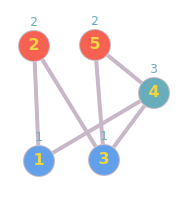
\includegraphics[width=0.4\textwidth]{figures6/GCol.png}
    \caption{G 3-coloreable}
    \end{subfigure}
    \caption{En la figura se colorea $G$ mediante la funci\'on $f= \left\{\begin{aligned} 1, &\ v \in \{1,3\}\\
                                                                                          2, &\ v \in \{2,5\} \\\
                                                                                          3, &\ v \in \{4\}\end{aligned}\right.$}
\end{figure} 

Observaciones:
\begin{itemize}
 \item $\chi(G) \leq |V(G)|$
 \item $\chi (K_n)=n$
 \item $\chi (C_{2k})=2$
 \item $\chi (C_{2k+1})=3$
 \item Si un grafo es bipartito es 2-coloreable
 \item El número cromático es la menor cantidad de conjuntos independientes que se pueden formar en G
 \item Si H es subgrafo de G entonces $\chi (H)\leq \chi (G)$
 \item $w(G)\leq \chi (G)$, donde w es el número de clique de G
\end{itemize}

\begin{dfn}[Grafo cr\'itico]
 Un grafo G es cr\'itico si para todo subgrafo propio H de G se cumple que el n\'umero 
 crom\'atico de H es menor que el n\'umero crom\'atico de G, o sea, $\chi (H)<\chi (G)$
\end{dfn}

\begin{dfn}[Grafo k-cr\'itico]
 Un grafo G es k-cr\'itico si es crítico y $\chi (G)=k$
\end{dfn}


\begin{dfn}[Grafo k-v\'ertice-cr\'itico]
 Un grafo G es k-v\'ertice-cr\'itico si su n\'umero crom\'atico es $k$ y $\forall v\in V(G)$ se tiene que $\chi (G-v)<\chi (G)$
\end{dfn}

\textbf{Nota:} $\chi (G-v)=k-1$

\begin{figure}[H]
    \centering
    \begin{subfigure}[b]{0.30\textwidth}
        \centering
        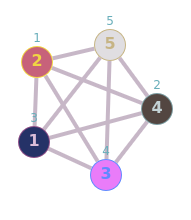
\includegraphics[width=0.4\textwidth]{figures6/k5Col.png}
        \caption{$K_n$ es n-cr\'itico}
    \end{subfigure} 
    \begin{subfigure}[b]{0.30\textwidth}
        \centering
        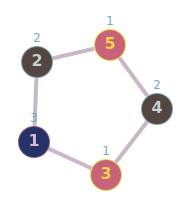
\includegraphics[width=0.4\textwidth]{figures6/C5Col.png}
        \caption{$C_{2p +1}$ es 3-cr\'itico}
    \end{subfigure}
    \begin{subfigure}[b]{0.30\textwidth}
        \centering
        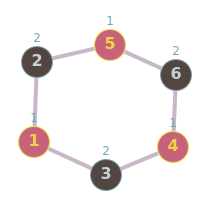
\includegraphics[width=0.4\textwidth]{figures6/C6Col.png}
        \caption{$C_{2p}$ nunca es k-cr\'itico}
    \end{subfigure}
\end{figure} 


\begin{teo}
 Si G es un grafo k-crítico con $k\geq 2$ entonces G es conexo y $\delta (G)\geq k-1$
\end{teo}

\begin{dem}[Reducci\'on al Absurdo]
 
\end{dem}


Demostremos que G es conexo

Suponga que G es k-crítico y no es conexo, entonces se descompone en t componentes conexas $c_1,c_2,\dots,c_t$, luego $k=max(\chi(c_1),\chi(c_2),\dots,\chi(c_t))$ por lo que existe un i tal que $1\leq i \leq t$ y $\chi(c_i)=k$ entonces es posible quitar cualquier vértice de cualquier componente conexa que no sea $c_i$ y se mantendría entonces $k=\chi(c_i)=max(\chi(c_1),\chi(c_2),\dots,\chi(c_t))$, por tanto G no sería k-crítico, lo que es una contradicción. Por tanto G es conexo.\\

Demostremos la segunda parte.

Supongamos que  $\delta (G)< k-1$, entonces sea $v\in V(G)$ tal que 

$deg(v)=\delta (G)$, por tanto tomemos G'=G-v. Como G es k-crítico entonces $\chi(G$´$)=\chi(G)-1$ o sea, se puede colorear a G' con k-1 colores

Si se pone de vuelta a v como $deg(v)<k-1$ entonces v tiene a lo sumo $k-2$ vértices adyacentes a él, que potencialmente tienen todos colores diferentes, como se dispone de k-1 colores, se puede colorear a v con un color que no tenga ninguno de sus adyacentes, luego es posible colorear a G con $k-1$ colores lo que es una contradicción. 

Por tanto, queda demostrado que si G es un grafo k-crítico con $k\geq 2$ entonces G es conexo y $\delta (G)\geq k-1 \ \blacksquare$

\begin{teo}
 Sea G un grafo tal que $\chi(G)=k$ entonces al menos k vértices de G tienen grado mayor o igual que $k-1$
\end{teo}

\begin{dem}
 
\end{dem}

Primeramente demostremos el siguiente Lema:
\begin{itemize}
    \item[]\textbf{Lema.}\textit{ Si $G$ es $k$-coloreable $\Rightarrow$ tiene un subgrafo $k-$cr\'itico.}

    \begin{dem}        
    \end{dem}
    Si G no es k-crítico entonces se puede suprimir un v\'ertice de $G$ tal que $G' = G-v$ siga cumpliendo que $\chi{G'} = k$. 
    Este procedimiento se repite, es decir si $G'$ no es $k-$cr\'itico se suprime otro v\'ertice que no modifique el n\'umero crom\'atico.
    Eventualmente se detiene este proceso pues no se puede hacer una eliminaci\'on infinita en los v\'ertices del grafo por \textbf{PBO}. Por tanto el grafo que se obtiene al terminar el procedimiento es un subgrafo $k-$critico de $G \ \blacksquare$
\end{itemize}

\begin{figure}[H]
    \centering
    \begin{subfigure}[b]{0.55\textwidth}
        \centering
        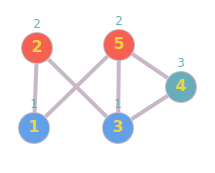
\includegraphics[width=0.4\textwidth]{figures6/otroGcol.png}
        \caption{$G$ 3-coloreable}
    \end{subfigure} 
    \begin{subfigure}[b]{0.35\textwidth}
        \centering
        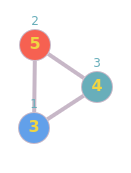
\includegraphics[width=0.4\textwidth]{figures6/3criticoSubG.png}
        \caption{Subgrafo $3$-cr\'itico de $G$}
    \end{subfigure}
    \caption{Ejemplo de subgrafo $k-$cr\'itico}
\end{figure} 
    
Sea $Q$ el subgrafo $k-$cr\'itico de $G$, que sabemos existe por \textbf{Lema}. $Q$ cumple que $\delta(Q)\geq k-1$ y tiene al menos k vértices. Luego el grado de cualquier vértices es igual o mayor que $k-1$
Como todos los v\'ertices de $Q$ tienen en $G$ un grado mayor o igual al que presentan en $Q$, se cumple que en $G$ hay al menos $k$ v\'etices con grado mayor o igual a $k-1 \ \blacksquare$

\begin{teo}
 Sea G un grafo, entonces $\chi(G)\leq 1 + \Delta(G)$
\end{teo}

\begin{dem}
Demostración por inducción en el número de vértices $n$. 
\end{dem}

\textbf{Caso base:} Para $n=1$ se tiene que $\chi(G)=1$ y $\Delta(G)=0$, luego $1\leq1+0$\\

\textbf{Paso inductivo:} Probemos que si se cumple que para un grafo $G$ con  $n$ v\'ertices que $\chi(G) \leq 1 + \Delta(G)$, entonces se cumple para un grafo de $n+1$ v\'ertices\\

Sea $G$ con $n+1$ vértices, si se tiene $G'=G-v$ entonces $G'$ tiene $n$ vértices luego
$\chi(G$´$)\leq 1 + \Delta(G$´$)$ pero $\Delta(G$'$)\leq \Delta(G)$\\ 
por tanto\\
$\chi(G$´$)\leq 1 + \Delta(G$´$)\leq 1 + \Delta(G) \  $\\

Luego es posible colorear a G' con $\Delta(G)+1$ colores distintos. Note que v a lo sumo tiene $\Delta(G)$ vértices adyacentes, como hay $\Delta(G)+1$ colores siempre puede colorearse v de modo que no tenga el mismo color que ninguno de sus adyacentes, por tanto es posible colorear a G con $\Delta(G)+1$ colores distintos, luego $\chi(G)\leq 1 + \Delta(G)$ $\blacksquare$\\


\textbf{Problema:} Cual es la menor cantidad de colores para representar un mapa, de modo que los territorios adyacentes tengan diferentes colores asignados.

\begin{figure}[H]
    \centering
    \begin{subfigure}[b]{0.55\textwidth}
        \centering
        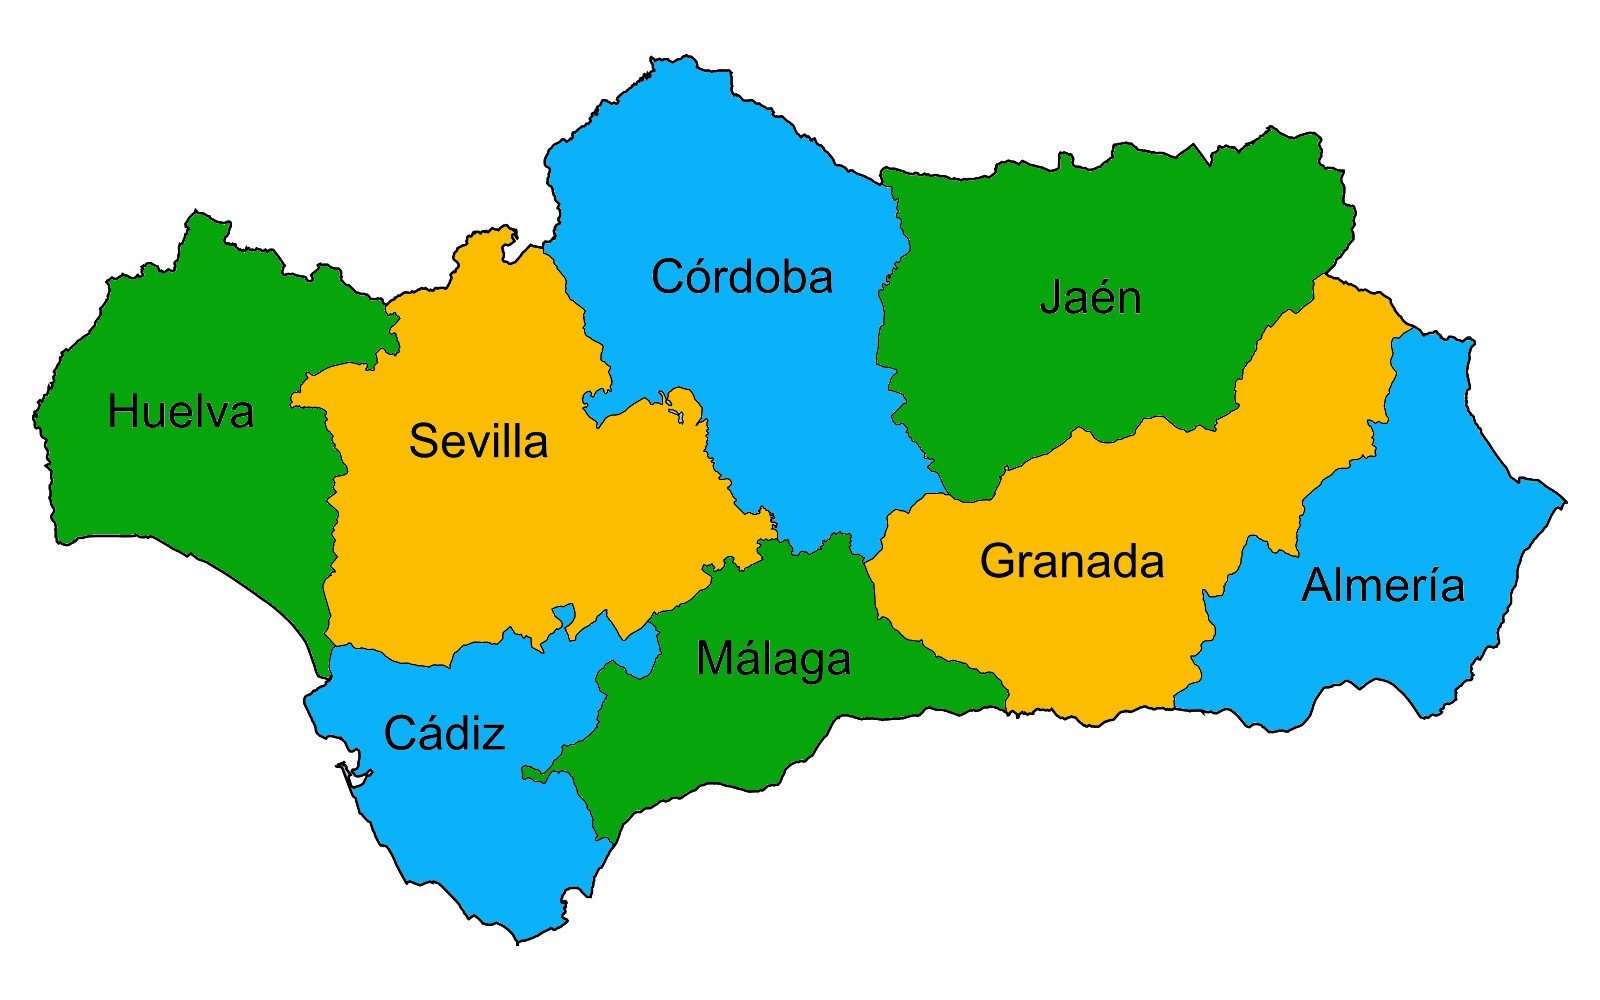
\includegraphics[width=\textwidth]{figures6/Andalucia_Coloreada.jpg}
    \end{subfigure} 
\end{figure} 

Dado un mapa, el grafo resultante de tomar un vértice en el centro de cada región y poner aristas
entre los vértices de regiones que se tocan entre sí, es planar. Por tanto el problema se resume en encontrar el n\'umero crom\'atico de un grafo planar.

\begin{figure}[H]
    \centering
    \begin{subfigure}[b]{0.55\textwidth}
        \centering
        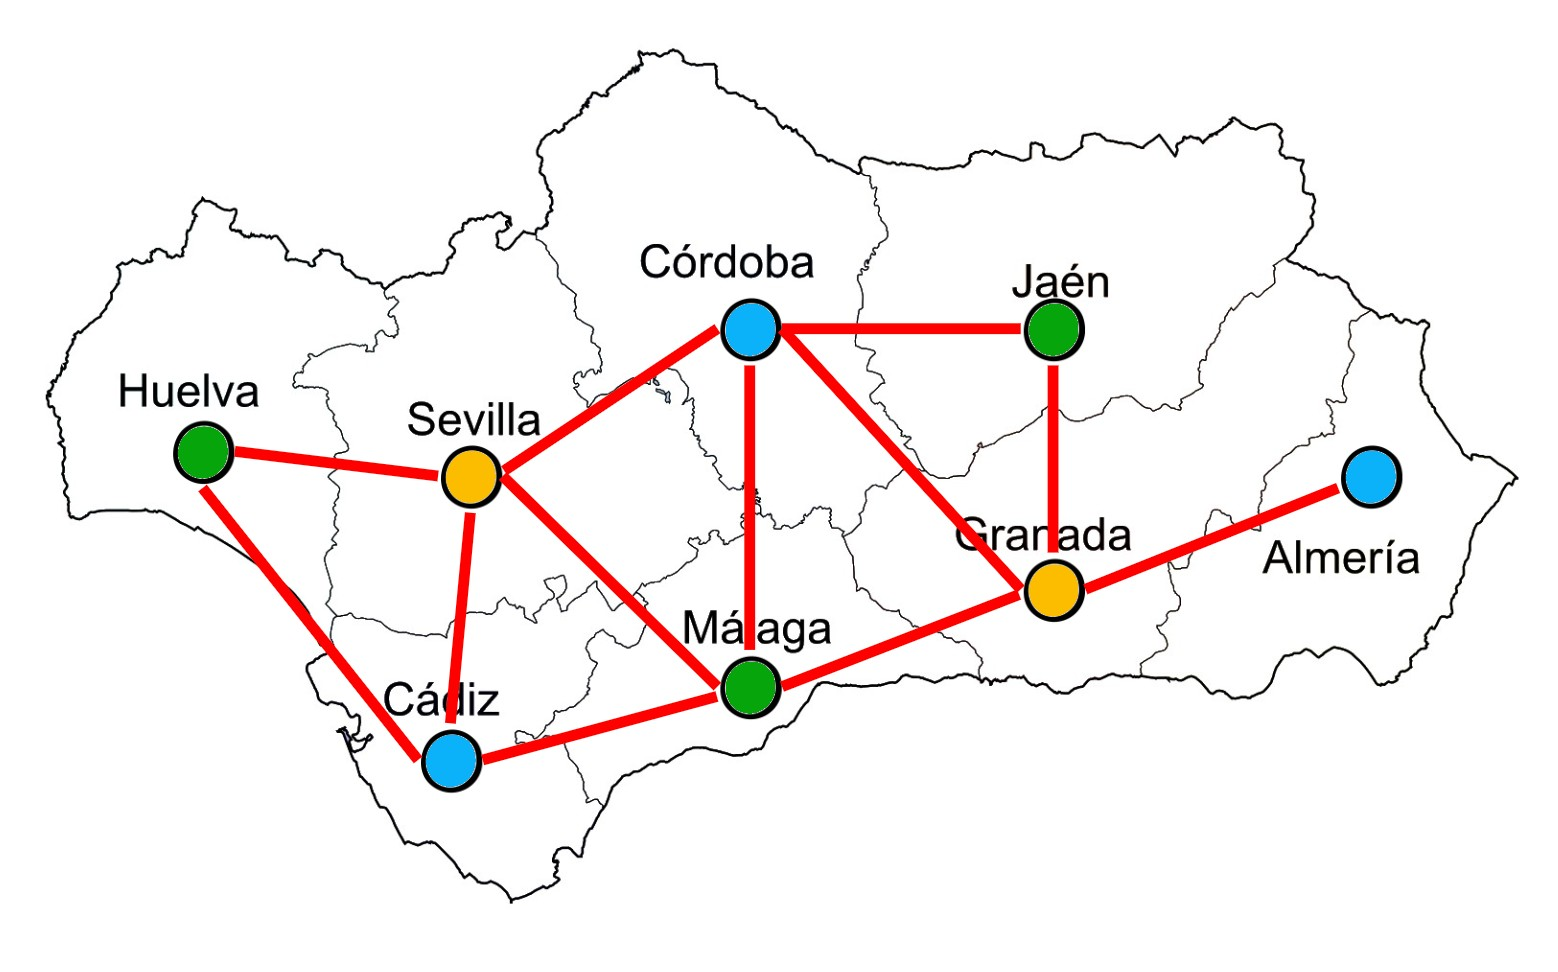
\includegraphics[width=\textwidth]{figures6/Grafo_Andalucia_Color.jpg}
    \end{subfigure} 
\end{figure} 

\begin{teo}
 Sea G un grafo planar entonces $\chi(G)\leq 6$
\end{teo}

\begin{dem}
Demostración por inducción en el número de v\'ertices.
\end{dem}

\textbf{Caso base:} Para $n=1$ es trivial que se necesita solo un color.

\textbf{Paso inductivo:} Probemos que si se cumple para n se cumple para n+1

Como $G$, con $n+1$ vértices, es planar tiene al menos un vértice cuyo grados es menor o igual a 5, digamoes que este vértice es v.

Tomemos el grafo G'=G-v, como G es planar entonces al quitar un vértice a este y dando G', G'continúa siendo planar. 

Como el número de vértices de G' es n y es planar, por hipótesis de inducción, se tiene que 
$\chi(G$'$)\leq 6$. Al reinsertar v, como $deg(v)\leq 5$, se tiene que v tiene a lo sumo 5 vértices adyacentes cuyos colores pueden ser todos potencialmente distintos, basta con colorear v con un color que no tengan sus vecinos, luego es posible colorear a G con 6 colores distintos $\blacksquare$.

\begin{teo}[Teorema de los 5 colores] El número cromático de un grafo planar es menor o igual que 5 
\end{teo}

\begin{dem}
Demostración por inducción en el número de vértices.
\end{dem}

\textbf{Caso Base:} $n< 5$ es trivial que se puede colorear con 5 colores.

\textbf{Hip\'otesis} Demostremos que si se cumple para un grafo de $n$ v\'ertices, entonces se cumple para uno de $n+1$

Ahora, como el grafo G es planar, tiene n+1 vertices, siempre hay un vértice con 5 o menos vértices adyacente, digamos que ese vértice es v. Entonces se tiene $G'= G-v$, con n vértices, que es 5-coloreable (por hipótesis de inducción)

Si $deg(v)\leq 4$ ya estaría demostrado. 
Si el $deg(v)=5$ pero sus vértices adyacentes solo usan, entre ellos, 4 colores también estaría demostrado.

Tendríamos que ver el caso con $deg(v)=5$ y sus adyacentes usan 5 colores.

Para ello %consideremos un disco $D$ (una ciscunferencia al de centro $v$) que abarque solo lo suficiente para contener las aristas adyacentes a $v$. 
llamaremos $v_1,v_2,v_3,v_4$ y $v_5$ a los vértices adayacentes a $v$ y los tendremos en ese mismo oreden en el sentido del giro de las agujas del reloj 
%en el disco $D$.

%Adem\'as sean las aristas $s_1,s_2,s_3,s_4$ y $s_5$, tales que $s_i = \{v, v_i\}$ y 
Como sabemos que cada v\'ertice tiene un color diferente de los $5$ colores que se utilizan en el grafo, sin p\'erdida de la generaldidad digamos que $c(v_i) = i$ (el color del v\'ertice $i-$\'esimo es $i$).

Cualquier camino $P$ que exista entre $v_1$ y $v_3$, conforma el ciclo $C = <v, v_1, P, v_3,v>$ que separa a los v\'ertices $v_2$ y $v_4$, los cuales caen en dos caras diferentes de $C$.

\begin{figure}[H]
    \centering
    \begin{subfigure}[b]{0.90\textwidth}
        \centering
        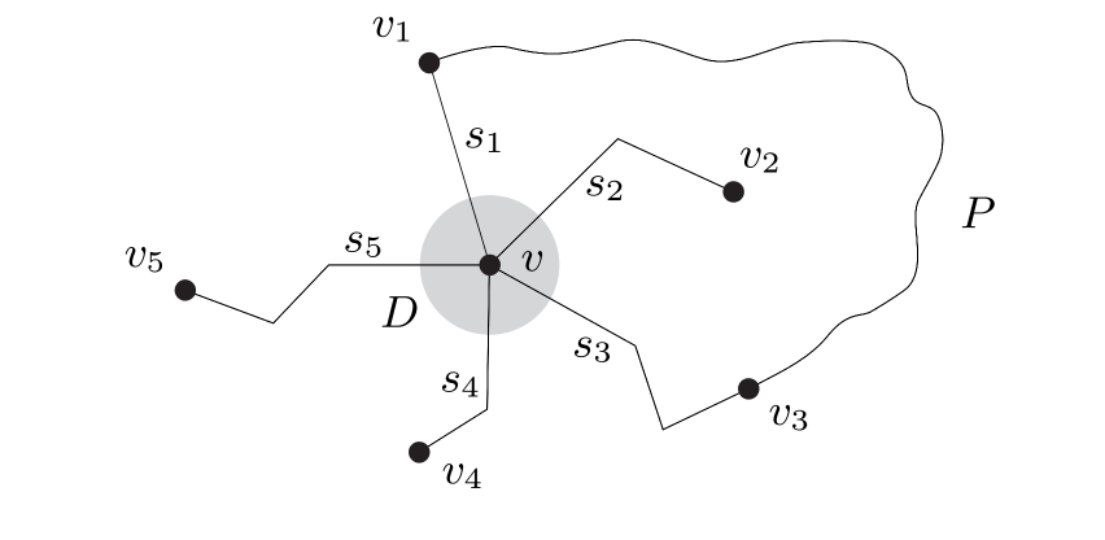
\includegraphics[width=0.7\textwidth]{figures6/5col.png}
    \end{subfigure} 
\end{figure} 

Consideremos entonces el subgrafo $H_{1,3}$, grafo inducido por aquellos v\'ertices de $G'$ tales que su color es $1$ o $3$, n\'otese que $v_1, v_3 \in H_{1,3}$. De este subgrafo analicemos todos los caminos que inician en $v_1$ y alternan entre los dos colores. Estos caminos forman una Componente Conexa dentro del grafo $H_{1,3}$ que por construcci\'on es bipartito.
Si ninguno de los caminos que inician en $v_1$ alcanza a $v_3$, entonces, es posible invertir el color de todos los v\'ertices involucrados en estos caminos, esto generar\'ia una bipartici\'on v\'alida en la cual a $v_1$ se le asigna el color $3$, donde quedar\'ia el color $1$ disponible para colorear al v\'ertice $v$.

\begin{figure}[H]
    \centering
    \begin{subfigure}[b]{0.30\textwidth}
        \centering 
        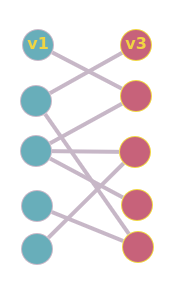
\includegraphics[width=0.4\textwidth]{figures6/recol1.png}
        \caption{$H_{1,3}$}
    \end{subfigure} 
    \begin{subfigure}[b]{0.50\textwidth}
        \centering 
        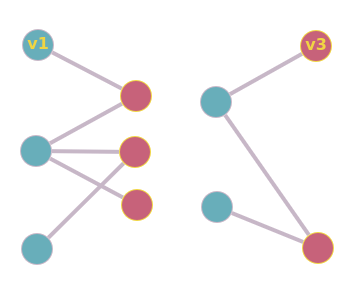
\includegraphics[width=0.4\textwidth]{figures6/recol2.png}
        \caption{Caminos que inician en $v_1$}
    \end{subfigure}
    \begin{subfigure}[b]{0.50\textwidth}
        \centering 
        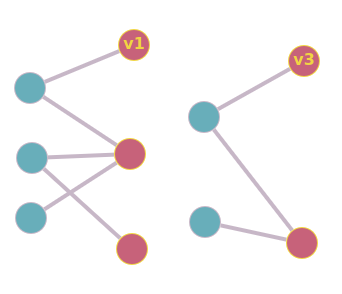
\includegraphics[width=0.4\textwidth]{figures6/recol3.png}
        \caption{Alternando color}
    \end{subfigure}
    \begin{subfigure}[b]{0.30\textwidth}     
        \centering    
        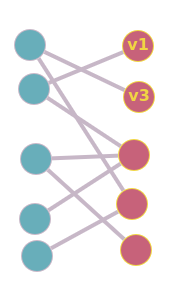
\includegraphics[width=0.4\textwidth]{figures6/recol4.png}
        \caption{Reconstruyendo $H_{1,3}$}
    \end{subfigure}
\end{figure} 

Si por otra parte, alguno de los caminos alternantes que inicien en $v_1$ llega a $v_3$, tomamos entonces el subgrafo $H_{2,4}$ de $G'$, que se conforma an\'alogo al anterior pero esta vez tomando los v\'ertices con color $2$ y $4$, en este caso, $v_2, v_4 \in H_{2,4}$. 

Si tomamos los caminos alternantes que inician en $v_2$ sabemos que ninguno puede terminar en $v_4$, porque sabemos que existe un camino $P$ alternante de v\'ertices de colores $1$, $3$ que separa a los v\'ertices $v_2$ y $v_4$ en dos regiones diferentes, por lo que cualquier camino de $v_2$ a $v_4$ tiene que pasar por alg\'un v\'ertice de color $1$ o $3$.

Entonces alternando los colores de los caminos que empiezan en $v_2$ de $H_{2,4}$, se tiene que ahora $v_2$ tiene color $4$, y el color $2$ queda disponible para pintar a $v$, de donde se puede pintar $G$ con $5$ colores $\blacksquare$.


\begin{teo}[Teorema de los 4 colores] El número cromático de un grafo planar es menor o igual que 4 
\end{teo}

La demostración del \textbf{Teorema de los 4 colores} se ha realizado con verficiación computacional combinando varias ideas teóricas.

\end{document} 
